\documentclass[e4_tp1_main.tex]{subfiles}
\begin{document}

\section{Topolog\'ia: Funcionamiento de una topolog\'ia y comprensio\'n de todas las curvas}

\subsection*{a)} 

Se diseñ\'o una fuente con las siguientes caracter\'isticas:

\begin{table}[H]
\centering
\begin{tabular}{|l|l|l|l|l|}
\hline
\multicolumn{1}{|c|}{Grupo}  & $V_{i}$ & $V_{o}$  & $\frac{\Delta V_{o_{max}}}{V_o}$ & $f_{sw}$ \\ \hline
3     						& 3.3V     & 5V  & 5\%   & 60kHz  \\ \hline
\end{tabular}
\label{tabla:datos de la fuente}
\end{table} 

Como se pide una tensi\'on de salida continua mayor que a la entrada, se utiliz\'o un convertidor boost. 

\begin{figure}[H]
  \centering
    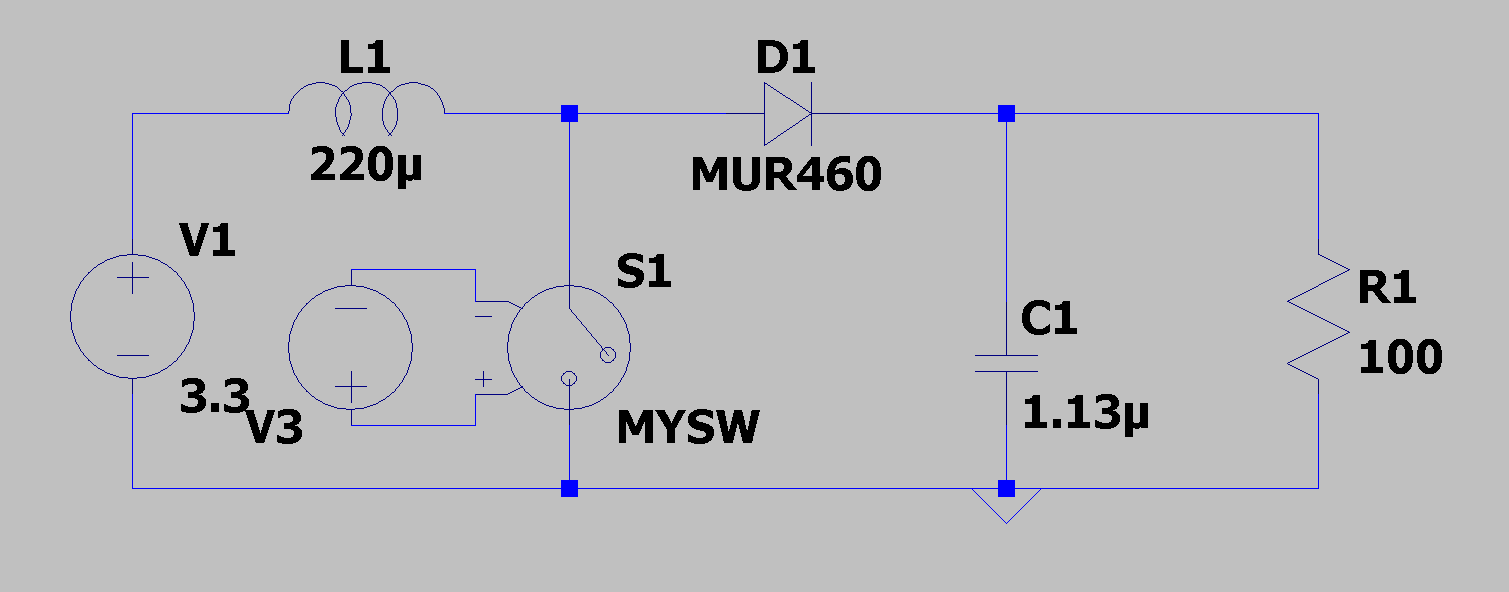
\includegraphics[scale = 0.5]{Imagenes/punto2/Circuito}
  \caption{Convertidor Boost}
  \label{fig:circuito pto 2}
\end{figure}

Sabemos que el duty cycle en este convertidor esta dado por: 
$$D_{ideal}=1-\frac{V_i}{V_o}=0.34$$

Con el valor del duty obtenemos el periodo de encendido de la llave $T_{on}=D T_s=D \frac{1}{f_{sw}}$


Para asegurarnos que estemos trabajando en modo continuo, elegimos una $I_{o}$ tal que: $I_{o}>I_{OB}$.

\begin{table}[H]
\centering
\begin{tabular}{|l|l|}
\hline
\multicolumn{1}{|c|}{$L [\mu H]$} & {$I_{OB} [mA]$}    \\ \hline
220                   & 14   \\ \hline
330                   & 9,35 \\ \hline
\end{tabular}
\caption{Calculo de $I_{OB}$ seg\'un el valor de $L$}
\label{tabla:calculo de Iob}
\end{table}

Por lo tanto, suponiendo $I_o=50mA$, obtenemos una carga de $R=100\Omega$



El valor del capacitor se obtuvo con la siguiente formula:
$$C=\frac{T_{on}}{R\frac{\Delta V_{o_{max}}}{V_o}}=1.13\mu F$$

Para realizar las simulaci\'on se eligi\'o  $L=220\mu H$ y se obtuvo que: 
$$D_{real}=0.43$$

\subsection*{b)}

Se realiz\'o el gr\'afico de la señal de disparo (SW), tensión en el inductor (VL),corriente en el inductor (IL) y corriente en el diodo (ID) considerando el diodo real. 

\begin{figure}[H]
  \centering
    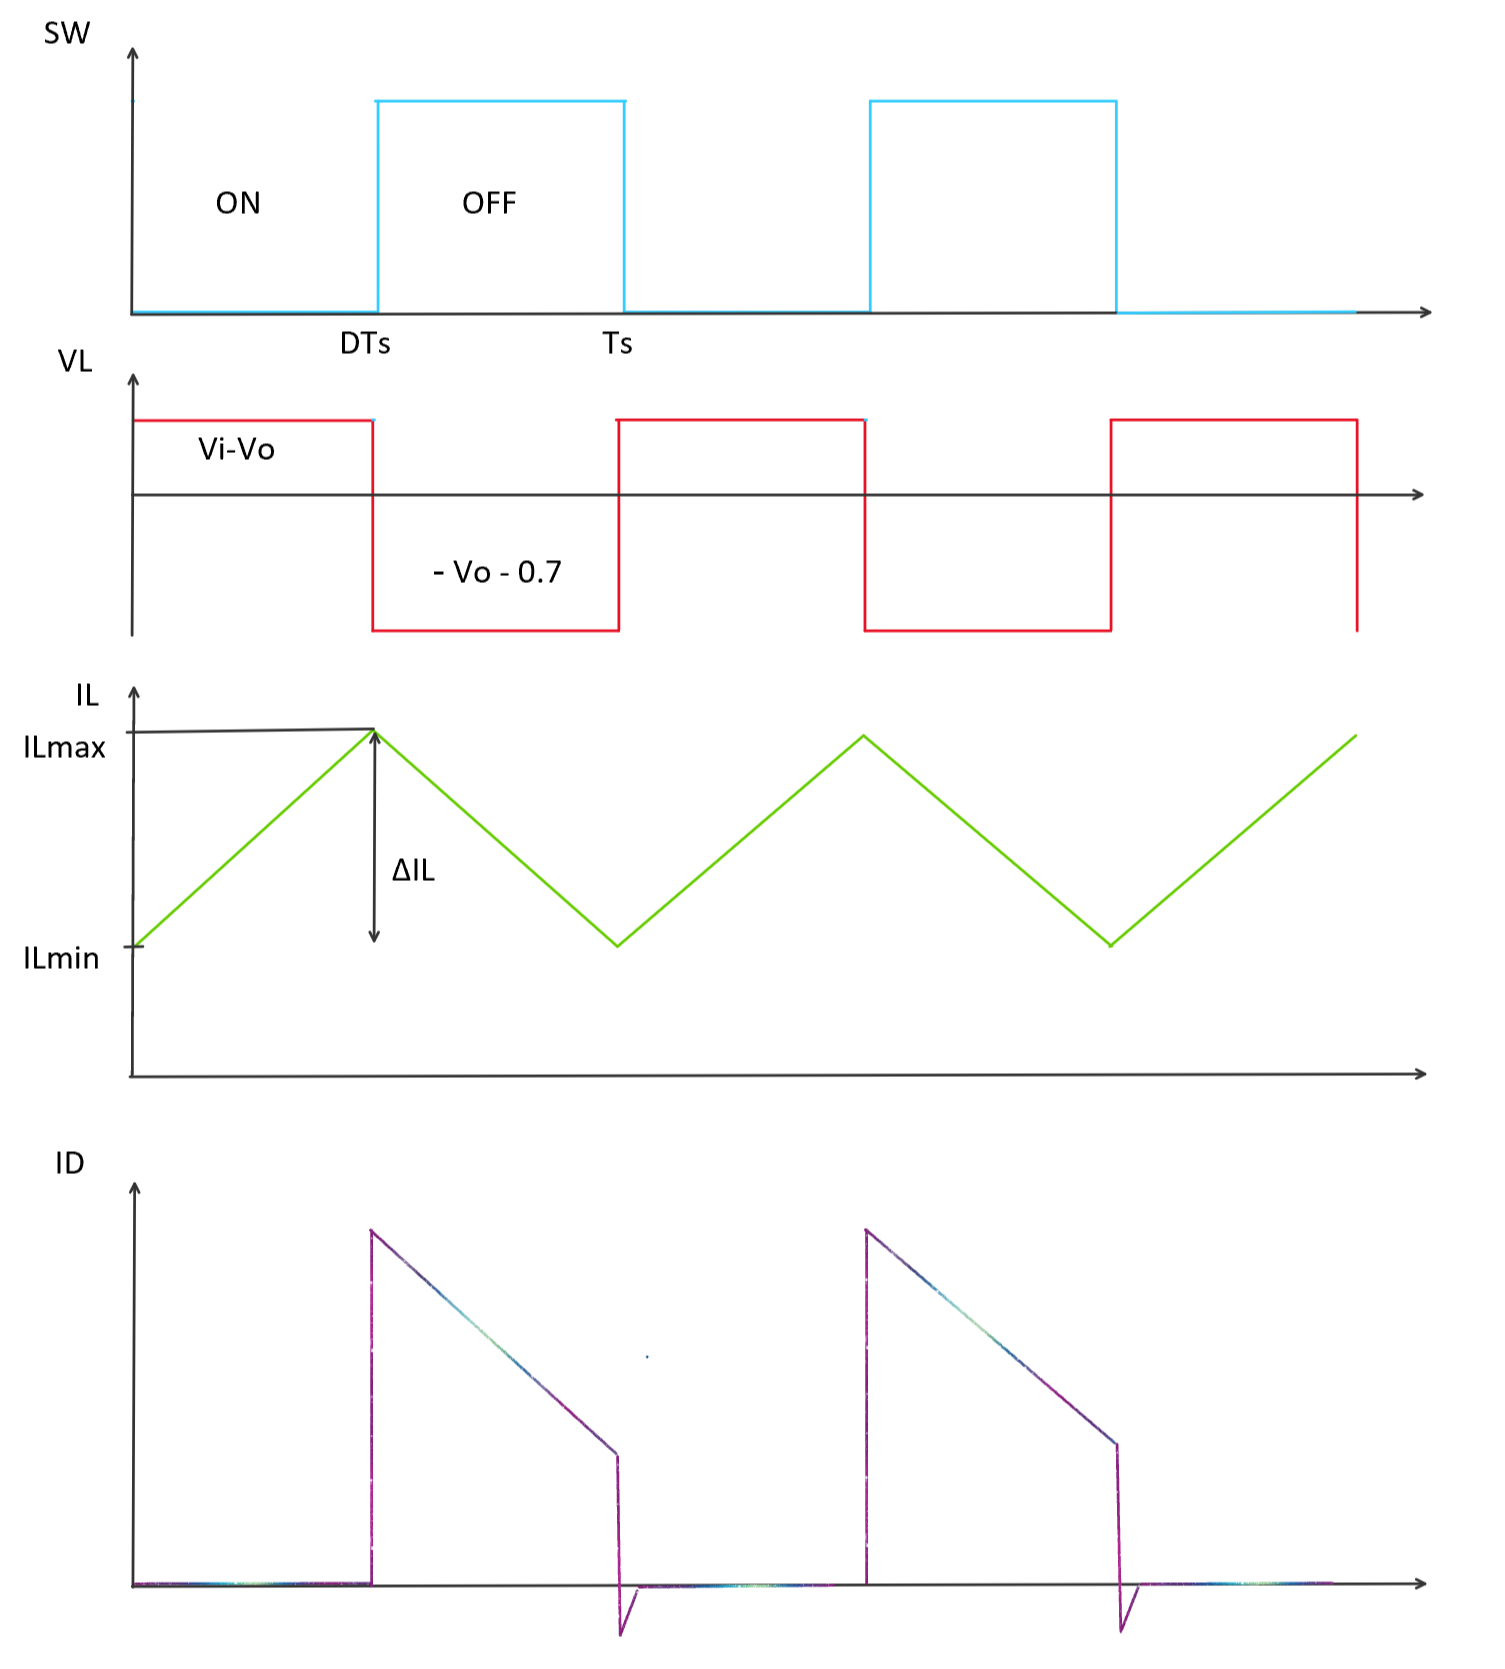
\includegraphics[scale = 0.7]{Imagenes/punto2/Dibujo}
  \caption{Gr\'afico las curvas de la topolog\'ia de convertidor boost}
  \label{fig:dibujo}
\end{figure}

\subsection*{c)}

A continuacion se mustra la simul\'on en LTspice las curvas del inciso anterior. 

\begin{figure}[H]
  \centering
    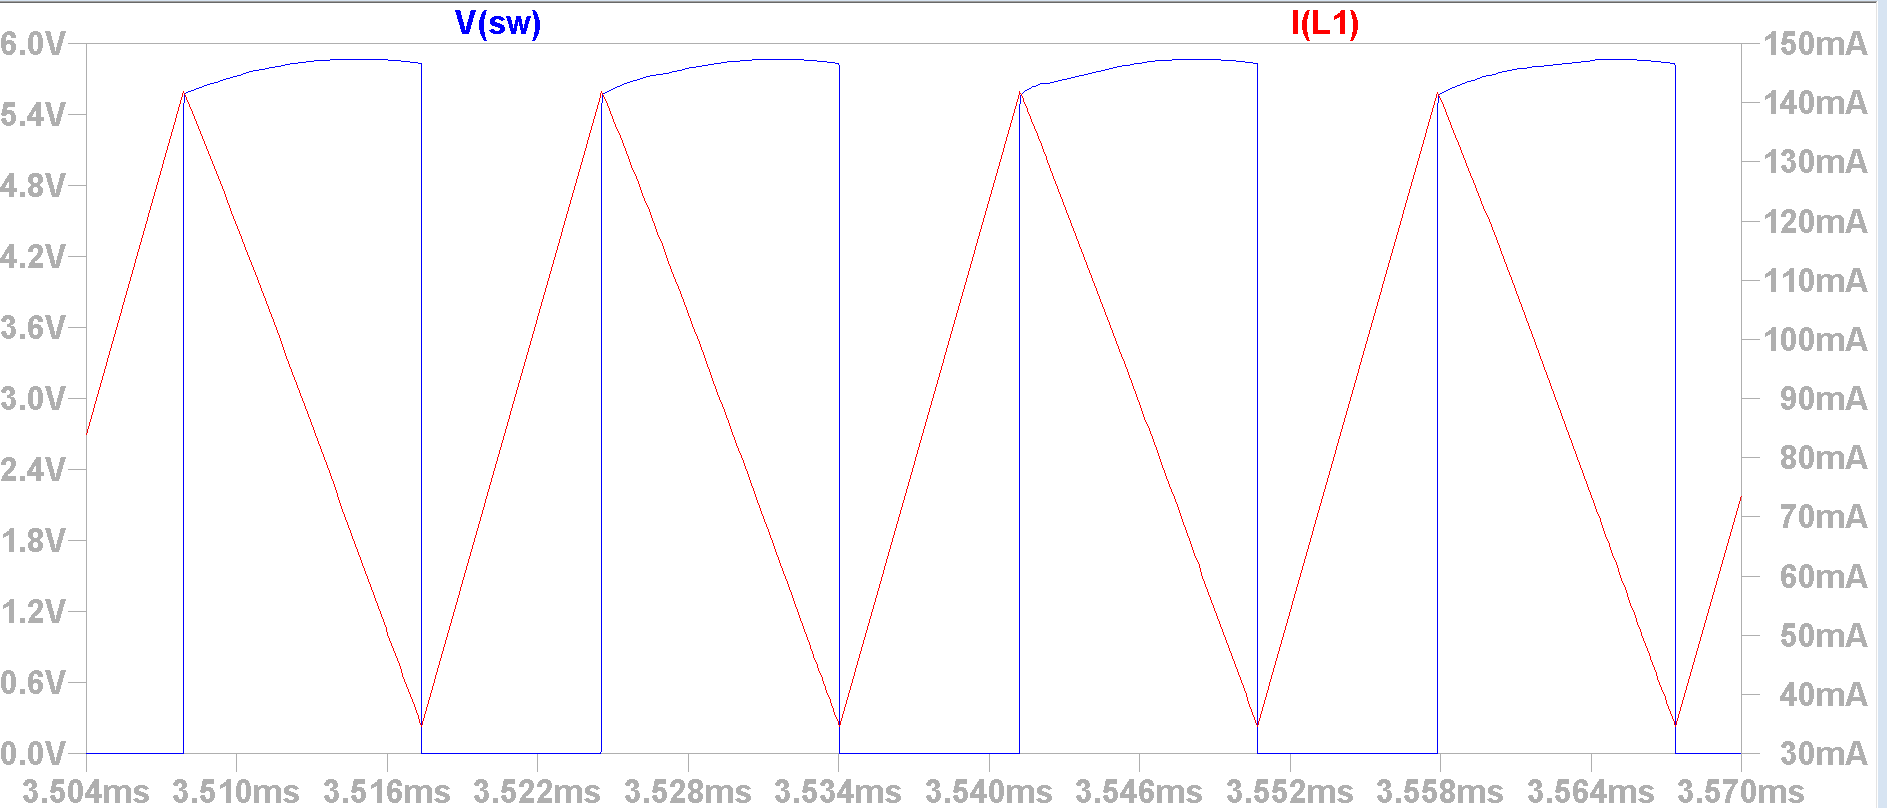
\includegraphics[scale = 0.4]{Imagenes/punto2/SW&IL}
  \caption{Simulaci\'on SW(azul) y IL(roja)}
  \label{fig:SW&IL}
\end{figure}


\begin{figure}[H]
  \centering
    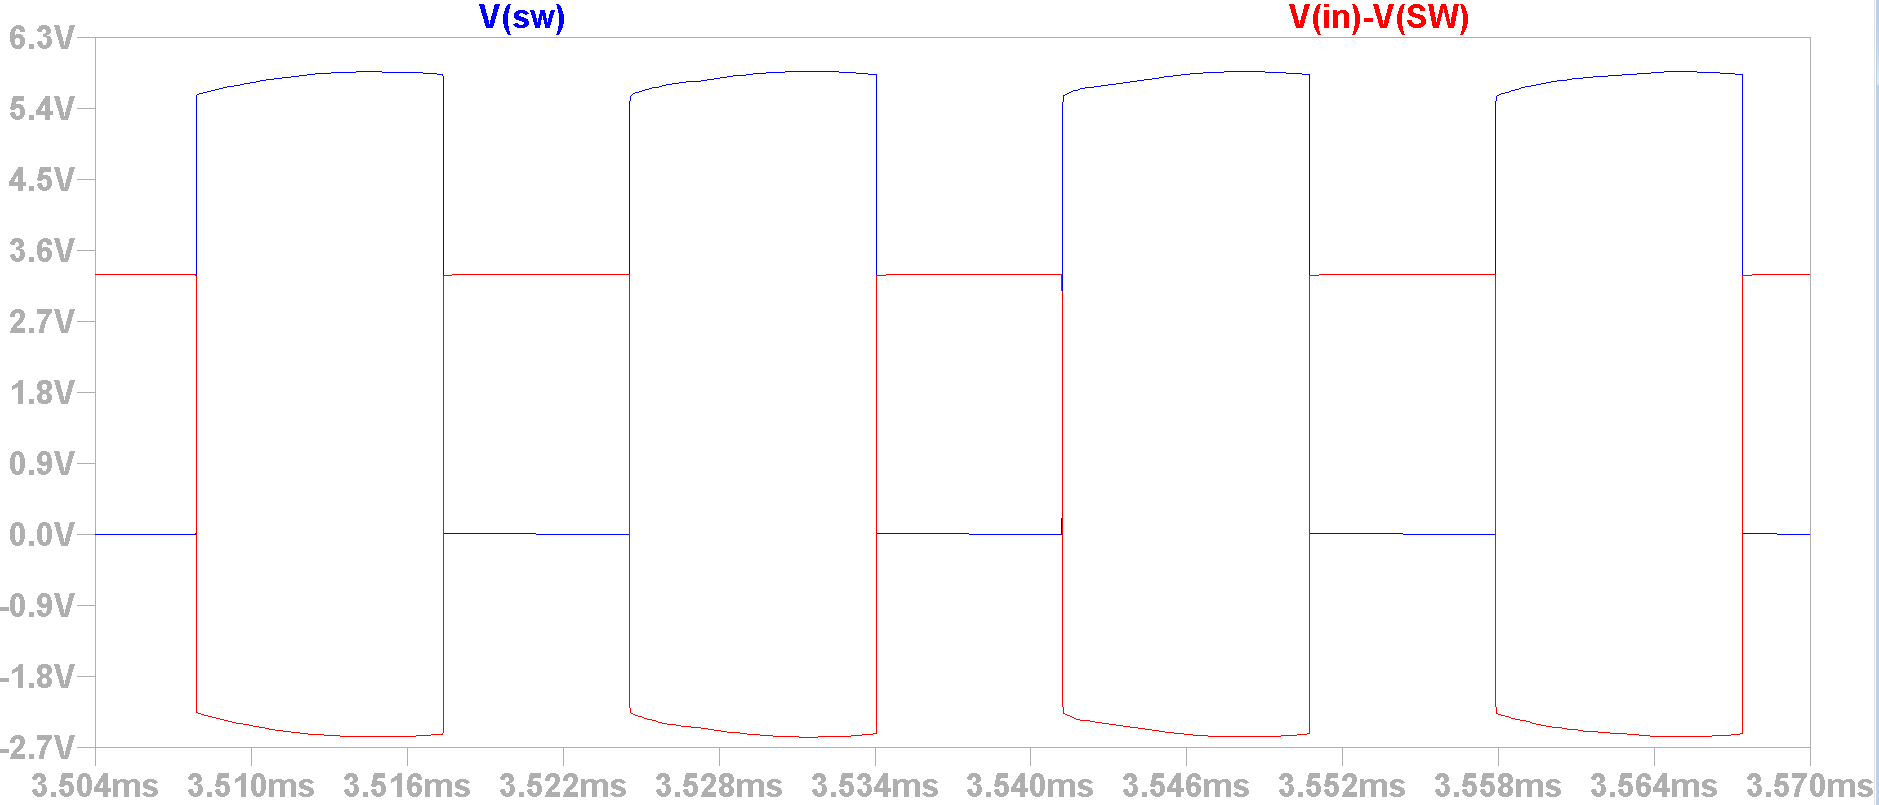
\includegraphics[scale = 0.4]{Imagenes/punto2/SW&VL}
  \caption{Simulaci\'on SW(azul) y VL(roja)}
  \label{fig:SW&VL}
\end{figure}


\begin{figure}[H]
  \centering
    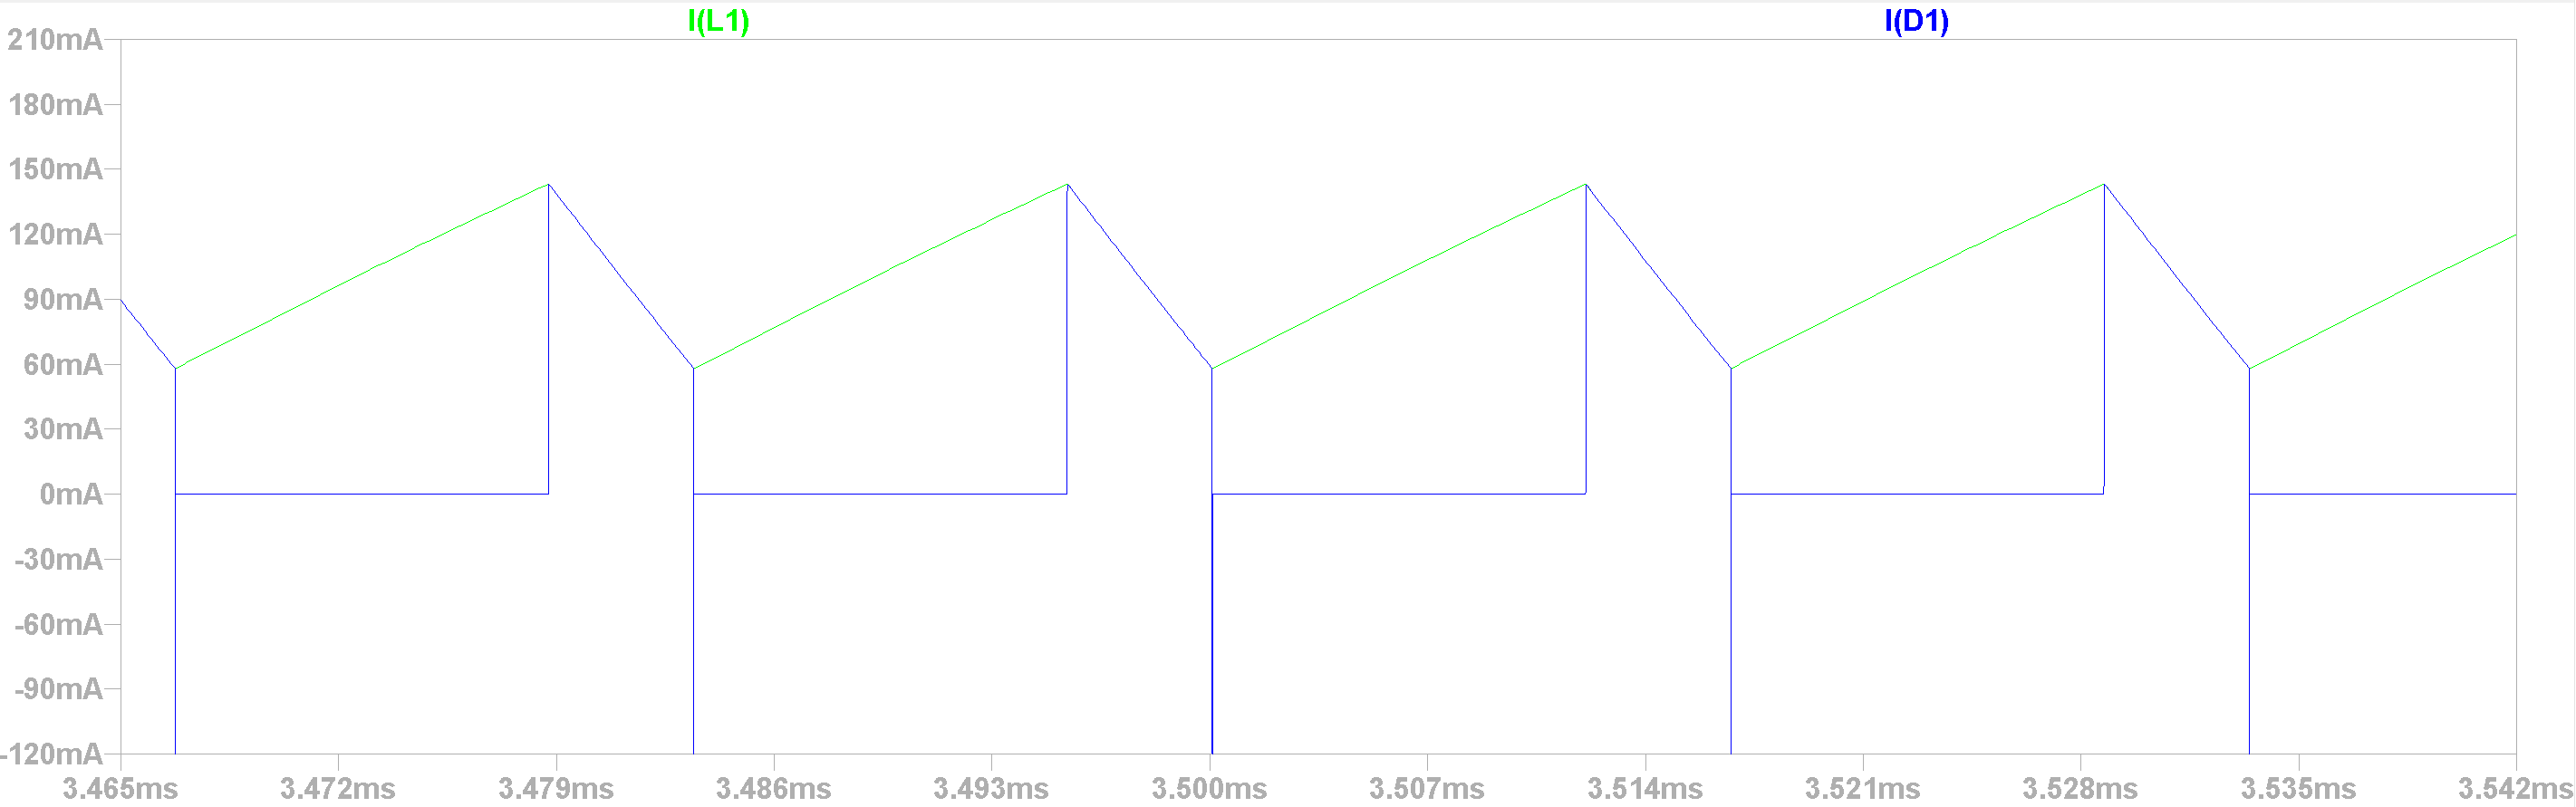
\includegraphics[scale = 0.52]{Imagenes/punto2/IL&ID}
  \caption{Simulaci\'on IL(verde) y ID(azul)}
  \label{fig:IL&ID}
\end{figure}


\subsection*{d)}





\newpage
\end{document}